\vspace{-2mm}
\section{Experiments}
\vspace{-2mm}
To understand how reasoning capabilities can be scaled in masked dLLMs through training adaptations, we conduct comprehensive experiments to answer the following main research questions:
\vspace{-1.5mm}
\begin{itemize}[leftmargin=15pt,topsep=0pt,itemsep=0.3pt,parsep=0pt]
    \item[(1)] How do SFT on reasoning traces and applying \grpo{} \textbf{\emph{independently}} improve LLaDA’s reasoning capabilities?
    \item[(2)] What additional gains can be achieved by \emph{combining} SFT and \grpo to create d1-LLaDA?
    \item[(3)] \textbf{Design Choices:} How does the proposed log-probability estimation with \emph{randomized masking} in \grpo{} and the masking probability $p_{\text{mask}}$ affect training efficiency and stability?
\end{itemize}


\subsection{Models, Tasks and Setups}
\textbf{Models} We employ LLaDA-8B-Instruct \citep{nie2025largelanguagediffusionmodels}, a state-of-the-art open-sourced dLLM that has not undergone post-training, as our primary experimental testbed and baseline. We apply 3 post-training recipes to LLaDA-8B-Instruct: (a) SFT, (b) \grpo, (c) d1: applying \grpo on the checkpoint after SFT, where we refer to them as LLaDA+SFT, LLaDA+\grpo, and d1-LLaDA, respectively. \looseness=-1

\textbf{Tasks} We conduct experiments on six reasoning tasks in three categories: (1) \textbf{Mathematical reasoning}: we use GSM8K \citep{cobbe2021training}, a dataset of multi-step grade school math problems, and MATH500~\citep{lightman2023lets}, a curated subset of 500 problems drawn from the MATH dataset~\citep{hendrycks2021measuring} comprising high-school competition math problems; (2) \textbf{Planning}: this includes two tasks: 4x4 Sudoku puzzles, which require constraint satisfaction and systematic elimination to fill a grid with numbers; and Countdown with 3 numbers, a combinatorial arithmetic game in which models must reach target numbers using basic arithmetic operations on a given set of numbers. (3) \textbf{Coding}: comprises of two benchmarks; HumanEval~\citep{chen2021evaluating}, a suite of 164 hand‑crafted Python algorithmic programming problems and MBPP~\citep{austin2021program}, a crowd‑sourced collection of 257 Python tasks.

\textbf{Training} For SFT, we train on s1k~\citep{muennighoff2025s1} for 20 epochs, with a sequence length of 4096. For RL, we train a separate model for each task. More specifically, for GSM8K, MATH500, we train on the training split; for Countdown and Sudoku, we train on synthetic generated datasets. We use a composed reward function that combines both formatting and correctness rewards. Due to the heavy computational cost of online generations, we limit the generation sequence length of online generations to be 256 throughout RL training. Other hyperparameters of training, training and evaluation datasets, reward functions, and inference setups are detailed in~\cref{appendix:training_details}.

% 7700, 6600 steps (number of gradient updates) respectively; for Countdown and Sudoku, we train on synthetic generated datasets for 5000, 3800 steps respectively.

\textbf{Evaluation} For all the benchmarks, we evaluate LLaDA-8B-Instruct and LLaDA+SFT on the final checkpoint for all the tasks. For LLaDA+\grpo and d1-LLaDA, we evaluate every 100 steps starting from step 600 and report the best results. We evaluate all models with 0-shot-prompting and greedy decoding with generation lengths of 128, 256 and 512 separately.


\begin{table}[t] 
\centering 
\caption{\textbf{Model performance on Mathematics and Planning Benchmarks:} \textbf{\textcolor{green!70!black}{Green values}} indicate best performance and \textbf{\textcolor{blue!60!black}{blue values}} indicate second-best performance. The results demonstrate that \textbf{d1-LLaDA} consistently outperforms other models, applying \grpo{} consistently improves the starting checkpoint, and \grpo alone shows better performance than SFT.} 
\vspace{2mm} 
\label{tab:performance_results} 
\scalebox{0.8}{ 
\begin{tabular}{l ccc ccc ccc ccc} 
\toprule 
& \multicolumn{3}{c}{\textbf{GSM8K }} & \multicolumn{3}{c}{\textbf{MATH500 }} & \multicolumn{3}{c}{\textbf{Countdown }} & \multicolumn{3}{c}{\textbf{Sudoku }} \\ 
\cmidrule(lr){2-4} \cmidrule(lr){5-7} \cmidrule(lr){8-10} \cmidrule(lr){11-13} 
\textbf{Model / Seq Len} & \textbf{128} & \textbf{256} & \textbf{512} & \textbf{128} & \textbf{256} & \textbf{512} & \textbf{128} & \textbf{256} & \textbf{512} & \textbf{128} & \textbf{256} & \textbf{512} \\ 
\midrule 
LLaDA-8B-Instruct & 68.7 & 76.7 & 78.2 & 26.0 & 32.4 & 36.2 & 20.7 & 19.5 & 16.0 & 11.7 & 6.7 & 5.5 \\ 
\midrule 
+ SFT & 66.5 & 78.8 & 81.1 & 26.2 & 32.6 & 34.8 & 20.3 & 14.5 & 23.8 & 16.5 & 8.5 & 4.6 \\ 
\midrule 
+ \grpo & \textcolor{blue!60!black}{72.6} & \textcolor{blue!60!black}{79.8} & \textcolor{blue!60!black}{81.9} & \textcolor{blue!60!black}{33.2} & \textcolor{blue!60!black}{37.2} & \textcolor{blue!60!black}{39.2} & \textcolor{blue!60!black}{33.2} & \textcolor{blue!60!black}{31.3} & \textcolor{blue!60!black}{37.1} & \textcolor{blue!60!black}{18.4} & \textcolor{blue!60!black}{12.9} & \textcolor{green!70!black}{\textbf{11.0}} \\ 
\midrule 
\makecell{+ SFT + \grpo \\(\textbf{d1-LLaDA})} & \textcolor{green!70!black}{\textbf{73.2}} & \textcolor{green!70!black}{\textbf{81.1}} & \textcolor{green!70!black}{\textbf{82.1}} & \textcolor{green!70!black}{\textbf{33.8}} & \textcolor{green!70!black}{\textbf{38.6}} & \textcolor{green!70!black}{\textbf{40.2}} & \textcolor{green!70!black}{\textbf{34.8}} & \textcolor{green!70!black}{\textbf{32.0}} & \textcolor{green!70!black}{\textbf{42.2}} & \textcolor{green!70!black}{\textbf{22.1}} & \textcolor{green!70!black}{\textbf{16.7}} & \textcolor{blue!60!black}{9.5} \\ 
\bottomrule 
\end{tabular} 
} 
\vspace{-2em} 
\end{table}



\subsection{Main Results}
\label{subsec:training}

\textbf{\grpo{} outperforms both LLaDA and SFT and improves over initialization checkpoint consistently .}  
\cref{tab:performance_results} reports the performance of baseline LLaDA-8B-Instruct and models obtained by different post-training recipes across four tasks using zero-shot evaluation, where each \grpo{} model was trained for each task. For each task, we evaluate with three generation sequence lengths, and \cref{fig:effective_len} plots the average number of effective tokens. We present the following predominent findings.

Both \grpo{} and SFT yield improvements over the LLaDA-8B-Instruct baseline, with \grpo{} demonstrating consistently larger gains. Specifically, \grpo{} outperforms both LLaDA-8B-Instruct and SFT, in all 12 setups, while SFT outperforms LLaDA-8B-Instruct in only 7 of them, demonstrating that \grpo{} achieves stronger overall performance than SFT alone. Both LLaDA+\grpo{} and d1-LLaDA demonstrate consistent improvements over their respective starting points. Specifically, LLaDA+\grpo{} outperforms the base LLaDA-8B-Instruct model across all setups, and d1-LLaDA surpasses LLaDA+SFT in every case. This indicates that \grpo{} provides reliable performance gains, regardless of the initialization—whether from a pretrained model or an SFT-adapted checkpoint.

\textbf{d1 recipe yields the highest gains.}  
SFT, followed by \grpo{}—resulting in d1-LLaDA—yields additional gains, beyond either method individually. This combined approach outperforms pure \grpo{} in 11 out of 12 setups, indicating a synergistic effect between the two training stages. Notably, while d1-LLaDA shows consistent improvements across all benchmarks, the magnitude varies by task: we observe modest improvements on GSM8K (3.9\%) and MATH500 (4.0\%), but significantly larger gains on Countdown (26.2\%) and Sudoku (10.0\%). We hypothesize this discrepancy stems from the base model's saturation on mathematical tasks, with less room for improvement as compared to planning benchmarks that involve structured constraint satisfaction patterns.

\begin{minipage}{0.45\textwidth}
\paragraph{Training a unified model across tasks retains strong performance.}
We train a single \grpo{} (and d1) model on the \emph{combined} GSM8K, MATH500, Countdown, and Sudoku datasets. To ensure balanced training, we subsample the data so that each task has the same number of training examples. Even with subsampling, \cref{tab:unified_performance_results} shows that \grpo{} scales well to multi-task settings without sacrificing accuracy compared to the per-task \grpo{} results in \cref{tab:performance_results}.

\vspace{1em}
\paragraph{Scaling \grpo to coding domains.} We also evaluate \grpo on coding tasks, where we train a model on the KodCode-Light-RL-10K dataset~\citep{xu2025kodcode}, which contains general coding tasks with solutions verified by synthetic unit tests. The \grpo{} results are shown in \cref{tab:coding_performance}. We find that \grpo consistently improves performance, regardless of the initialization point. Interestingly, our findings suggest that s1k is not suitable for coding, since it \textbf{lacks datapoints with code}. Exploration into finding the optimal SFT dataset is left for future works.
\end{minipage}
\hfill
\begin{minipage}{0.5\textwidth}
\captionof{table}{\textbf{Unified Model Performance Across Reasoning Tasks:} For \grpo and d1-LLaDA variants, a single model was trained on the combined dataset of GSM8K, MATH500, Countdown, and Sudoku. \textbf{\textcolor{green!70!black}{Green}} and \textbf{\textcolor{blue!60!black}{blue values}} indicate the best and second-best performance.} 
\label{tab:unified_performance_results} 
\scalebox{0.56}{ 
\begin{tabular}{l cc cc cc cc}
\toprule
& \multicolumn{2}{c}{\textbf{GSM8K}} & \multicolumn{2}{c}{\textbf{MATH500}} & \multicolumn{2}{c}{\textbf{Countdown}} & \multicolumn{2}{c}{\textbf{Sudoku}} \\
\cmidrule(lr){2-3} \cmidrule(lr){4-5} \cmidrule(lr){6-7} \cmidrule(lr){8-9}
\textbf{Model / Seq Len} & \textbf{128} & \textbf{256} & \textbf{128} & \textbf{256} & \textbf{128} & \textbf{256} & \textbf{128} & \textbf{256} \\
\midrule
LLaDA-8B-Instruct & 68.7 & 76.7 & 26.0 & 32.4 & 20.7 & 19.5 & 11.7 & 6.7 \\
\midrule
+ SFT (s1k) & 66.5 & \textcolor{blue!60!black}{78.8} & 26.2 & 32.6 & 20.3 & 14.5 & 16.5 & 8.5 \\
\midrule
+ combined \grpo & \textbf{\textcolor{blue!60!black}{72.4}} & 78.2 & \textbf{\textcolor{green!70!black}{30.2}} & \textbf{\textcolor{green!70!black}{36.6}} & \textcolor{blue!60!black}{27.7} & 19.5 & \textbf{\textcolor{green!70!black}{22.9}} & \textbf{\textcolor{green!70!black}{15.7}} \\
\midrule
\makecell{combined \textbf{d1-LLaDA}} & \textbf{\textcolor{green!70!black}{75.1}} & \textbf{\textcolor{green!70!black}{81.1}} & \textcolor{blue!60!black}{29.8} & \textcolor{blue!60!black}{35.4} & \textbf{\textcolor{green!70!black}{30.1}} & \textbf{\textcolor{green!70!black}{32.8}} & \textcolor{blue!60!black}{21.9} & \textcolor{blue!60!black}{15.4} \\
\bottomrule
\end{tabular}
}

\vspace{0.5em}
\captionof{table}{\textbf{Effectiveness of \grpo{} on Coding Benchmarks:} Evaluated with and without \grpo{} on HumanEval and MBPP. \grpo{} consistently improves over initialization checkpoint on coding tasks.}
\label{tab:coding_performance}
\scalebox{0.6}{ 
\begin{tabular}{l ccc ccc}
\toprule
 & \multicolumn{3}{c}{\textbf{HumanEval}} & \multicolumn{3}{c}{\textbf{MBPP}} \\
\cmidrule(lr){2-4} \cmidrule(lr){5-7}
\textbf{Model / Seq Len} & \textbf{128} & \textbf{256} & \textbf{512} & \textbf{128} & \textbf{256} & \textbf{512} \\
\midrule
\textbf{LLaDA-8B-Instruct}                     & 27.4 & 35.3 & 37.8 & 36.2 & 41.2 & 40.4 \\
\quad + \grpo                                  & 29.3 & 39.0 & 34.8 & 42.0 & 45.5 & 41.6 \\
\rowcolor{gray!10}
\quad $\Delta$ (\grpo{} gain)                  & \textbf{\textcolor{blue!60!black}{+1.9}} & \textbf{\textcolor{blue!60!black}{+3.7}} & \textbf{\textcolor{red!60!black}{-3.0}} & \textbf{\textcolor{blue!60!black}{+5.8}} & \textbf{\textcolor{blue!60!black}{+4.3}} & \textbf{\textcolor{blue!60!black}{+1.2}} \\
\midrule
\textbf{LLaDA-8B-Instruct + SFT (s1k)}         & 21.3 & 32.3 & 32.9 & 40.1 & 39.7 & 41.2 \\
\quad + \grpo                                  & 31.1 & 32.9 & 37.8 & 40.5 & 44.7 & 42.8 \\
\rowcolor{gray!10}
\quad $\Delta$ (\grpo{} gain)                  & \textbf{\textcolor{blue!60!black}{+9.8}} & \textbf{\textcolor{blue!60!black}{+0.6}} & \textbf{\textcolor{blue!60!black}{+4.9}} & \textbf{\textcolor{blue!60!black}{+0.4}} & \textbf{\textcolor{blue!60!black}{+5.0}} & \textbf{\textcolor{blue!60!black}{+1.6}} \\

\bottomrule



\end{tabular}
}
\end{minipage}


\vspace{1em}
\textbf{\grpo{} improves reasoning beyond training sequence length.}  
Although our \grpo{} training uses fixed sequence length of 256 for online generations, we observe performance gains at other generation sequence lengths as well. The improvements at 128 and 512 sequence lengths suggest that the model has learned more general reasoning strategies rather than overfitting to a specific length. This is further supported by the effective token usage data, presented in \cref{fig:effective_len}, which shows no truncation at 128 tokens and increased token utilization at 512.



\subsection{Discussion}
\textbf{Qualitative results show ``aha moments'' in SFT and d1-LLaDA generations.} While the performance for generation sequence length 128 and 256 increases with SFT, \grpo and d1 as compared to LLaDA-8B-Instruct, qualitatively, we do not observe significant differences in the generated reasoning traces. However, at sequence length 512, we begin observing ``aha moments'' in the SFT and d1-LLaDA models, which demonstrates self-correction and backtracking behaviors. We show these in \cref{appendix:qualitative}. For the same questions from GSM8k, we show generations of each model, with the variants using SFT showing self-verifications and self-corrections to the right answer. 
Our intuition is that the model has instilled behaviors such as verification of intermediate results and backtracking from the reasoning traces of s1k during the SFT stage.

\textbf{Sequential scaling with increasing generation sequence lengths.} LLaDA-8B-Instruct, SFT, \grpo and d1-LLaDA demonstrate improved performance with increasing sequence lengths for GSM8k and MATH500, with larger jumps observed from 128 to 256 ($\sim7.1\%$), than from 256 to 512 ($\sim2.5\%$). Qualitative examples in \cref{appendix:qualitative} show more sophisticated reasoning traces emerge with 512-token generation lengths. These findings align with previous research showing that increasing test-time compute through longer reasoning processes leads to improved performance in autoregressive models \citep{muennighoff2025s1}. However, we notice a mixed scaling trend on Countdown and Sudoku. Performance decreases with increasing sequence lengths for Sudoku across all models. For Countdown, LLaDA-8B-Instruct decreases monotonically with sequence length, while SFT, \grpo{} and d1-LLaDA peak at 512 sequence length. This likely stems from extensive searching requirements, beyond LLaDA-8B-Instruct's capabilities. We hypothesize favorable sequential scaling will strengthen with more robust base dLLMs. Unlike AR models like DeepSeek R1~\citep{guo2025deepseek}, we observe no significant CoT length growth post-RL training, as LLaDA-8B-Instruct was pre-trained on sequences up to 4096 tokens. Further scaling requires larger generation lengths during RL training, currently infeasible due to slow generation speed. Future research should develop efficient inference algorithms for online sampling to scale dLLM RL training.


\begin{figure}[t]

    \centering

    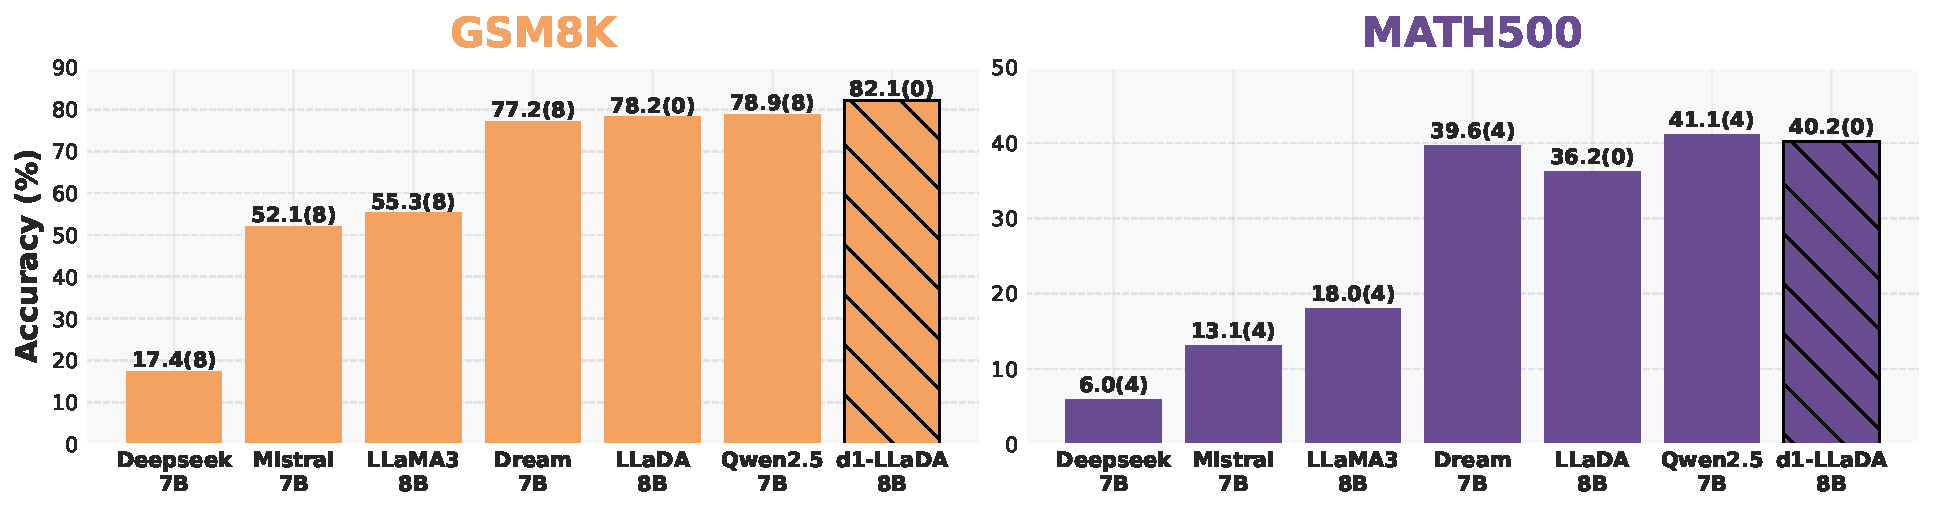
\includegraphics[width=0.75\linewidth]{figs/sota_comparison_dual_axis.pdf}

   \caption{\textbf{Comparison with state-of-the-art dLLMs and AR LLMs of similar size:} d1-LLaDA achieves the highest GSM8K score and the second-highest MATH500 score. LLaDA results are from our evaluation using 0-shot. Scores for other models are from Dream~\citep{dream2025}, using 8-shot prompts for GSM8K and 4-shot for MATH. Note that here we report d1-LLaDA with task-specific RL training.}

    \label{fig:enter-label}

\end{figure}


\begin{figure}[t]
    \centering
    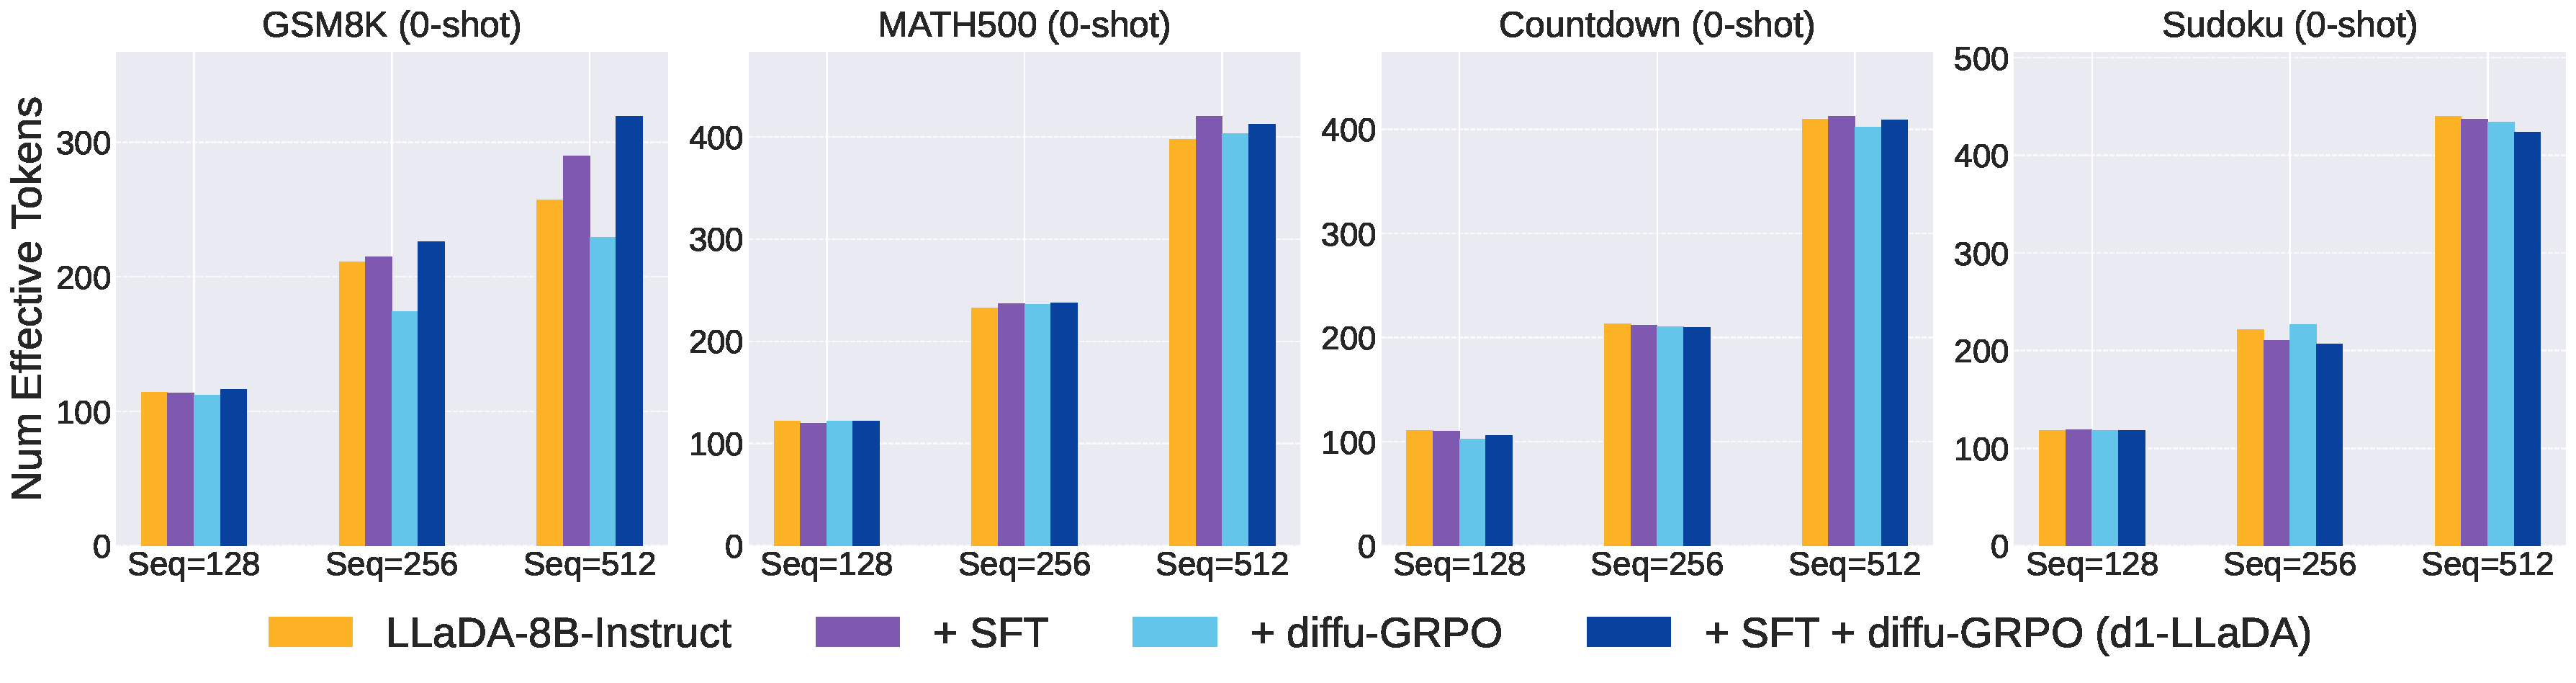
\includegraphics[width=0.8\linewidth]{figs/token_usage_single_row_plots.pdf}
    \caption{\textbf{Effective Token Usage:} As we increase the evaluation generation length, the number of effective tokens (average number of non-padding, non-EOS tokens per generation across tasks) grows and remains comparable for all the methods on MATH500, Countdown and Sudoku tasks. }
    \label{fig:effective_len}
\end{figure}

% \begin{table}[]
%     \centering
% \caption{Effective Tokens Usage: Average number of non-padding, non-EOS tokens per generation across tasks. While countdown and sudoku show minimal changes, GSM8K and MATH500 demonstrate improved token utilization with d1-LLaDA. \textcolor{green!70!black}{Green} indicates highest token usage and \textcolor{red!70!black}{red} indicates lowest token usage in each column.}
%         \vspace{2mm}
% \scalebox{0.76}{
% \begin{tabular}{l ccc ccc ccc ccc}
% \toprule
% & \multicolumn{3}{c}{\textbf{GSM8K }} & \multicolumn{3}{c}{\textbf{MATH500 }} & \multicolumn{3}{c}{\textbf{Countdown }} & \multicolumn{3}{c}{\textbf{Sudoku }} \\
% \cmidrule(lr){2-4} \cmidrule(lr){5-7} \cmidrule(lr){8-10} \cmidrule(lr){11-13}
% \textbf{Model / Seq Len} & \textbf{128} & \textbf{256} & \textbf{512} & \textbf{128} & \textbf{256} & \textbf{512} & \textbf{128} & \textbf{256} & \textbf{512} & \textbf{128} & \textbf{256} & \textbf{512} \\
% \midrule
% LLaDA-8B-Instruct & 114.4 & 211.0 & 256.8 & 122.2 & 232.4 & 397.8 & \textcolor{green!70!black}{110.7} & \textcolor{green!70!black}{213.0} & 409.8 & 117.9 & 221.5 & \textcolor{green!70!black}{439.8} \\
% \midrule 
% + SFT & 113.8 & 214.9 & 289.5 & \textcolor{red!70!black}{119.8} & 236.8 & \textcolor{green!70!black}{420.0} & 110.3 & \textcolor{red!70!black}{211.5} & \textcolor{green!70!black}{412.3} & \textcolor{green!70!black}{119.3} & \textcolor{red!70!black}{210.7} & 437.1 \\
% \midrule 
% + \grpo & \textcolor{red!70!black}{112.2} & \textcolor{red!70!black}{173.9} & \textcolor{red!70!black}{229.1} & 122.0 & 236.3 & 403.2 & \textcolor{red!70!black}{102.8} & 210.5 & \textcolor{red!70!black}{402.1} & 118.0 & \textcolor{green!70!black}{226.5} & \textcolor{red!70!black}{433.7} \\
% \midrule 
% \makecell{+ SFT + \grpo \\(\textbf{d1-LLaDA})} & \textcolor{green!70!black}{116.5} & \textcolor{green!70!black}{225.8} & \textcolor{green!70!black}{319.1} & \textcolor{green!70!black}{122.2} & \textcolor{green!70!black}{237.8} & 412.6 & 106.0 & 209.4 & 408.8 & \textcolor{green!70!black}{118.3} & 206.8 & 423.7 \\
% \bottomrule
% \end{tabular}
% }
% \label{tab:effective_len}
% \end{table}










\label{subsec:scaling}
\vspace{-2mm}
\subsection{Design Choices and Ablations for \grpo}
\label{subsec:exp_grpo}




\textbf{Random Masking for Likelihood Estimation Offers Implicit Regularization} Our randomized masking mechanism provides significant advantages for training masked dLLMs. As shown in Figure~\ref{fig:mu_ablation}, random masking consistently outperforms fixed masking across different values of policy optimization updates ($\mu$). While conventional approaches typically limit $\mu$ to 2 due to diminishing returns and overfitting risks, our approach enables scaling $\mu$ to much higher values (12, or even 24) while maintaining or improving performance, facilitating faster convergence of RL training. Consequently, fewer number of generations are needed, which in turn remarkably reduces the computational cost. The rightmost plot demonstrates the real-world efficiency gains, where models with higher $\mu$ values achieve better correctness rewards in significantly lesser wall clock time. 
This efficiency stems from creating diverse views of the input data during each optimization step, allowing the model to prevent in-batch overfitting and extract more learning signal from each generation.

\begin{figure}[t!]
 \centering
  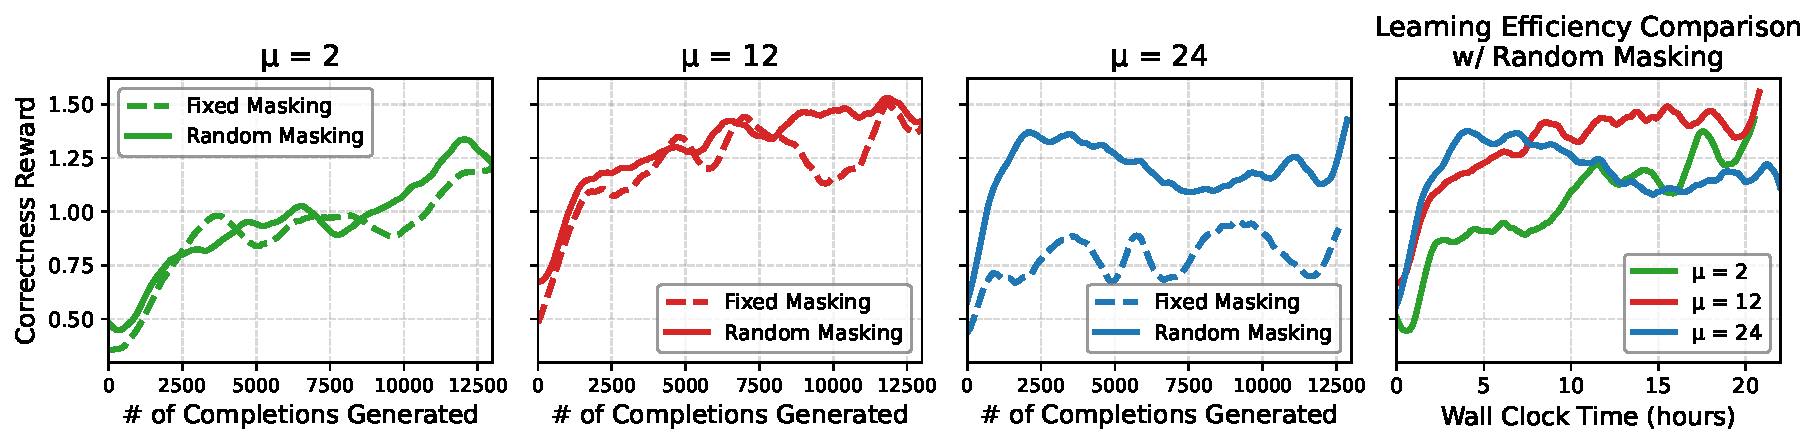
\includegraphics[width=0.86\textwidth]{figs/masking_strategy_comparison_first22hours_t0-22.pdf}
 \caption{\textbf{Comparison of fixed vs. random masking} across different policy optimization update values ($\mu$). The first three figures show GSM8K correctness reward vs. the number of completions generated during RL training with different $\mu$. Random masking consistently outperforms fixed masking. The rightmost panel compares all three $\mu$ values with random masking in terms of wall clock time, indicating higher efficiency from higher $\mu$ values.}
 \label{fig:mu_ablation}
\end{figure}


\begin{figure}[h!]
    \begin{minipage}{0.29\textwidth}
        \centering
        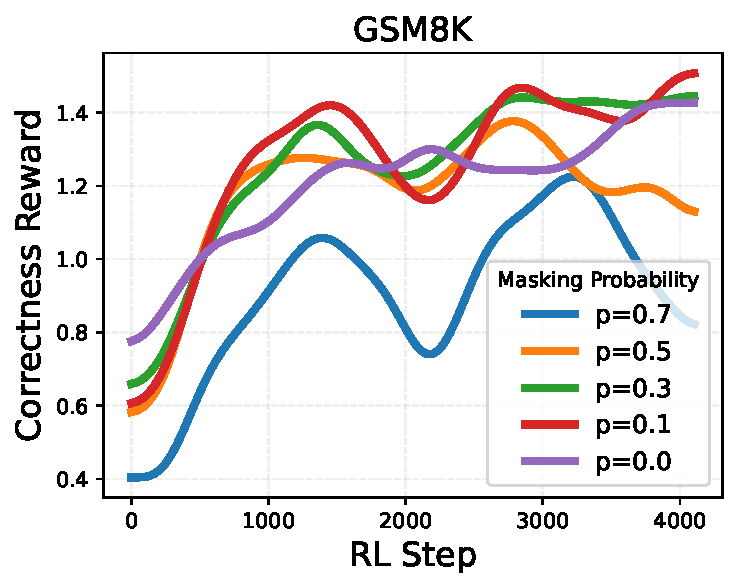
\includegraphics[width=0.98\textwidth]{figs/gsm8k_reward_trends_smooth_with_variance.pdf}
    \end{minipage}%
    \begin{minipage}{0.7\textwidth}
        \vspace{-1.5em}
\caption{\textbf{Ablation of prompt masking probability ($p_{\text{mask}}$)} on GSM8K reward trends. Light masking (0.1, 0.3) improves stability and performance over no masking (0.0), suggesting the regularization benefit of random masking as discussed in Sec~\ref{sec:method_grpo}. Higher masking rates (0.5, 0.7) introduce instability in later training stages.}

        
        \label{fig:p_mask}
    \end{minipage}
    \vspace{-2mm}
\end{figure}

\textbf{Effect of Masking Rate on Training Stability and Performance} We examine how prompt masking probability $p_{\text{mask}}$ influences \grpo{} training. As shown in Figure~\ref{fig:p_mask}, lower rates (0.1, 0.3) yield more stable training and better final performance by preserving more context tokens without masking them, while higher rates (0.5, 0.7) introduce instability, with 0.7 causing sharp degradation after 3000 steps. Although $p_{\text{mask}}=0.0$ avoids variability, it underperforms slightly, confirming the  regularization effect brought by random masking as discussed in Sec.~\ref{sec:method_grpo}. This effect is especially beneficial at large policy iteration counts ($\mu=12$), as used in this ablation.
